\chapter{Elektronische spectra en magnetisme van complexen}\label{ch:b3:complex-spectra-magnetism}

Robijn is rood en smaragd is groen, en toch danken beide hun kleur aan
hetzelfde ion, \ce{Cr^{3+}}, dat enkele aluminiumionen vervangt in twee
verschillende oxiden: korund,
$\ce{Al2O3}$, voor de robijn, het beryllium-aluminiumsilicaat beryl voor de
smaragd. In beide zit het chroom in een octaëder van zuurstofatomen; in
beryl is de octaëder iets groter en het ligandveld iets zwakker, en de
absorptiebanden van het ion verschuiven met ongeveer duizend golfgetallen
naar het rood. Dat volstaat om de doorgelaten kleur van rood naar groen
te veranderen. Dit hoofdstuk verklaart zulke spectra kwantitatief: hoe de
termen van een vrij ion in een ligandveld opsplitsen, hoe
\omterm{def:b3:complex-spectra-magnetism:tanabe-sugano}{tanabe-suganodiagrammen} twee bandposities omzetten in de
ligandveldsplitsing en de elektronenafstoting, waarom sommige banden
intens zijn en andere zwak, waarom sommige complexen vervormen, en hoe
magnetisme de ongepaarde elektronen telt.

\begin{recall}
Het deel van jaar~2 behandelde de overgangselementen en hun configuraties
$d^n$, de kristalveldsplitsing $\Delta_{\mathrm o}$, hoogspin- en laagspincomplexen, de
paringsenergie, de kristalveldstabilisatie-energie, $d$--$d$-overgangen, de
spectrochemische reeks, de ligandveldtheorie, en paramagnetische en
diamagnetische stoffen.
\Cref{ch:b3:many-electron-atoms} leidde de termsymbolen en de regels van
Hund af,
\cref{ch:b3:group-theory-applied} reduceerde representaties en
directe producten,
\cref{ch:b3:electronic-spectroscopy} formuleerde de spinselectieregel en
de \omterm{thm:b3:electronic-spectroscopy:laporte}{regel van Laporte} en beschreef \omterm{def:b3:electronic-spectroscopy:charge-transfer}{ladingsoverdrachtsovergangen}, en
\cref{ch:b3:partition-functions} gaf de \omterm{def:b3:partition-functions:boltzmann}{boltzmannverdeling}.
\end{recall}

\begin{omfigure}
\begin{minipage}[b]{0.3\linewidth}\centering
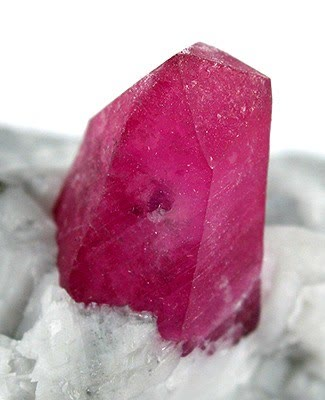
\includegraphics[height=4.2cm]{images/book4/ruby-crystal.jpg}\par
{\small robijn}
\end{minipage}\hspace{1.5em}
\begin{minipage}[b]{0.3\linewidth}\centering
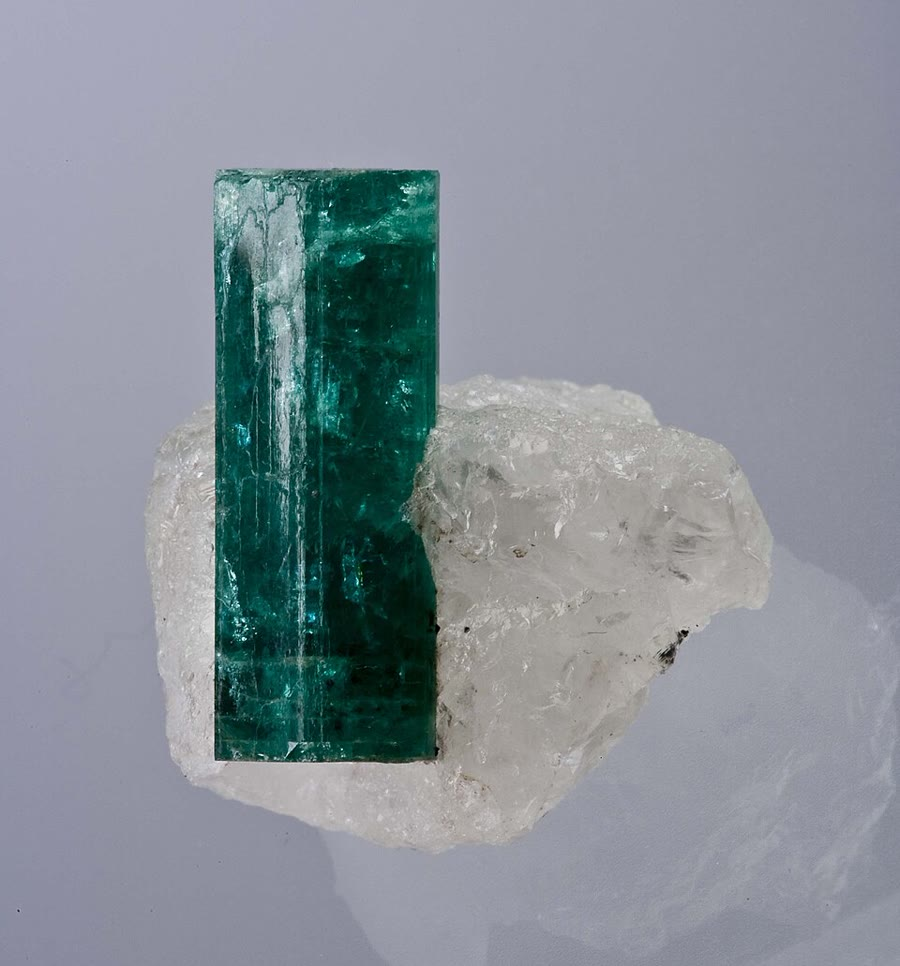
\includegraphics[height=4.2cm]{images/book4/emerald-crystal.jpg}\par
{\small smaragd}
\end{minipage}

{\small Een robijnkristal in marmer en een smaragdkristal op kwarts. In
beide komt de kleur van enkele procent \ce{Cr^{3+}} op een octaëdrische
plaats.}
\end{omfigure}

\section{Van termen van het vrije ion naar ligandveldtermen}

In een vrij ion splitst de elektronenafstoting een $d^n$-configuratie op in termen
($^4$F, $^4$P, $^2$G\dots\ voor $d^3$, \cref{ch:b3:many-electron-atoms}). In een complex wordt elke term
verder gesplitst door de liganden, en de niveaus worden benoemd met de
\omterm{def:b3:point-groups:irrep}{irreducibele representaties} van de \omterm{def:b3:point-groups:point-group}{puntgroep} van het complex.

\begin{definition}[Ligandveldterm]\label{def:b3:complex-spectra-magnetism:ligand-field-term}
Een \emph{ligandveldterm}\index{ligandveldterm} van een complex is een
verzameling ontaarde meerelektronentoestanden, benoemd met hun
\omterm{def:b3:many-electron-atoms:term}{spinmultipliciteit} en met de \omterm{def:b3:point-groups:irrep}{irreducibele representatie} van de \omterm{def:b3:point-groups:point-group}{puntgroep}
waartoe hun orbitaal deel behoort, zoals $^4$A$_{2g}$ of $^4$T$_{1g}$ in een octaëdrisch complex.
\end{definition}

\begin{proposition}[Karakters van de rotatiegroep]\label{prop:b3:complex-spectra-magnetism:rotation-characters}
De $2L+1$ toestanden van een term met baanimpulsmoment $L$ vormen een
representatie van de rotaties waarvan het \omterm{def:b3:point-groups:representation}{karakter} voor een rotatie over $\alpha$ gelijk is aan
\[
  \chi_L(\alpha) = \frac{\sin\bigl((L + \tfrac12)\alpha\bigr)}{\sin(\alpha/2)}, \qquad \chi_L(0) = 2L + 1 .
\]
\end{proposition}

\admitted

\begin{theorem}[Opsplitsing van de termen van het vrije ion in een octaëdrisch veld]\label{thm:b3:complex-spectra-magnetism:term-splitting}
In een octaëdrisch veld splitsen de termen van een $d^n$-ion op in
\begin{center}
\begin{tabular}{ll}
\hline
term van het vrije ion & octaëdrische termen (zelfde \omterm{def:b3:many-electron-atoms:term}{spinmultipliciteit}) \\ \hline
S & A$_{1g}$ \\
P & T$_{1g}$ \\
D & E$_g$ + T$_{2g}$ \\
F & A$_{2g}$ + T$_{1g}$ + T$_{2g}$ \\
G & A$_{1g}$ + E$_g$ + T$_{1g}$ + T$_{2g}$ \\ \hline
\end{tabular}
\end{center}
\end{theorem}

\begin{proof}
De octaëdrische groep is de rotatiegroep $O$ maal de inversie; de functies $d$
zijn even, dus elke term van een $d^n$-configuratie is even ($g$), en het volstaat te
reduceren in $O$, met de klassen $E$, $8C_3$, $3C_2$ ($=C_4^2$), $6C_4$ en $6C_2'$. Met de
propositie geldt voor $L = 3$: $\chi = 7$, $\sin(420^\circ)/\sin60^\circ = 1$, $\sin(630^\circ)/\sin90^\circ = -1$, $\sin(315^\circ)/\sin45^\circ = -1$
en $-1$. De \omterm{def:b3:point-groups:irrep}{karaktertabel} van $O$ (rijen $A_1$: 1, 1, 1, 1, 1; $A_2$: 1, 1, 1, $-1$, $-1$; $E$: 2,
$-1$, 2, 0, 0; $T_1$: 3, 0, $-1$, 1, $-1$; $T_2$: 3, 0, $-1$, $-1$, 1) en de \omterm{thm:b3:group-theory-applied:reduction}{reductieformule} van
\cref{ch:b3:group-theory-applied} geven $n(A_2) = (7 + 8 - 3 + 6 + 6)/24 = 1$, $n(T_1) = (21 + 3 - 6 +
6)/24 = 1$, $n(T_2) = (21 + 3 + 6 - 6)/24 = 1$, en nul voor $A_1$ en $E$. De andere rijen
volgen op dezelfde manier ($L = 0$: $(1, 1, 1, 1, 1)$; $L = 1$: $(3, 0, -1, 1, -1)$; $L = 2$: $(5, -1, 1,
-1, 1)$; $L = 4$: $(9, 0, 1, 1, 1)$).
\end{proof}

\begin{method}[Een term van het vrije ion opsplitsen]\label{met:b3:complex-spectra-magnetism:split-term}
\begin{enumerate}
  \item Zoek de grondterm van het vrije ion (regels van Hund) en de
        aangeslagen termen met dezelfde multipliciteit.
  \item Lees hun octaëdrische componenten af in de tabel; de
        \omterm{def:b3:many-electron-atoms:term}{spinmultipliciteit} verandert niet.
  \item Rangschik ze: voor de grondterm F van $d^2$, $d^7$ (hoogspin) is T$_{1g}$ de laagste;
        voor $d^3$, $d^8$ is het A$_{2g}$ (volgende propositie).
\end{enumerate}
\end{method}

\begin{proposition}[Gaten en de tetraëdrische omkering]\label{prop:b3:complex-spectra-magnetism:hole}
De termen van $d^{10-n}$ in een octaëdrisch veld zijn die van $d^n$ in omgekeerde
energievolgorde; de termen van $d^n$ in een tetraëdrisch veld zijn die van $d^{10-n}$ in een octaëdrisch
veld (zonder de indices $g$).
\end{proposition}

\begin{proof}
Een configuratie $d^{10-n}$ is gelijkwaardig met $n$ positieve gaten in een volle schil: de
gaten voelen de ligandveldpotentiaal met het tegengestelde teken, zodat
elke eenelektronsplitsing, en dus elke termsplitsing, omgekeerd wordt (de
elektronenafstoting tussen gaten is dezelfde als tussen elektronen). Een
tetraëdrisch veld heeft het tegengestelde teken van een octaëdrisch (de orbitalen $e$
liggen lager) en geen symmetriecentrum: $d^n$ in $T_d$ gedraagt zich als $d^n$ in een omgekeerd
veld, d.w.z.\ als $d^{10-n}$ in $O_h$.
\end{proof}

\begin{definition}[Correlatiediagram]\label{def:b3:complex-spectra-magnetism:correlation}
Een \emph{correlatiediagram}\index{correlatiediagram} verbindt de
toestanden van een systeem in twee grenssituaties, hier de termen van het
vrije ion, gesplitst door een zwak veld, en de configuraties $t_{2g}^ae_g^b$ van een sterk veld, waarbij
toestanden van dezelfde symmetrie verbonden worden zonder dat twee ervan
elkaar kruisen.
\end{definition}

\begin{omfigure}
\begin{tikzpicture}[font=\small]
  % free ion
  \pic (F) at (0,0) {omlevel={}{1.1}};
  \pic (P) at (0,3.0) {omlevel={}{1.1}};
  \node[anchor=east] at (F-l) {$^3$F};
  \node[anchor=east] at (P-l) {$^3$P};
  % weak field
  \pic (a) at (2.6,-0.8) {omlevel={}{1.0}};
  \pic (b) at (2.6,0.3) {omlevel={}{1.0}};
  \pic (c) at (2.6,1.4) {omlevel={}{1.0}};
  \pic (d) at (2.6,3.1) {omlevel={}{1.0}};
  \foreach \n/\t in {a/T$_{1g}$, b/T$_{2g}$, c/A$_{2g}$, d/T$_{1g}$(P)}{\node[omsymlabel, anchor=south] at (\n-c) {$^3$\t};}
  \draw[omcorr] (F-r) -- (a-l) (F-r) -- (b-l) (F-r) -- (c-l) (P-r) -- (d-l);
  % strong field configurations
  \pic (A) at (7.4,-1.6) {omlevel={}{1.0}};
  \pic (B) at (7.4,1.4) {omlevel={}{1.0}};
  \pic (C) at (7.4,1.9) {omlevel={}{1.0}};
  \pic (D) at (7.4,4.6) {omlevel={}{1.0}};
  \node[anchor=west] at (A-r) {$^3$T$_{1g}$ \quad $t_{2g}^2$};
  \node[anchor=west] at (B-r) {$^3$T$_{2g}$};
  \node[anchor=west] at (C-r) {$^3$T$_{1g}$ \quad $t_{2g}e_g$};
  \node[anchor=west] at (D-r) {$^3$A$_{2g}$ \quad $e_g^2$};
  \draw[omcorr] (a-r) -- (A-l) (b-r) -- (B-l) (c-r) -- (D-l) (d-r) -- (C-l);
  \node[anchor=north] at (0,-2.0) {vrij ion};
  \node[anchor=north] at (2.6,-2.0) {zwak veld};
  \node[anchor=north] at (7.4,-2.0) {sterk veld};
  \draw[->, black!50] (3.7,-2.3) -- (6.2,-2.3) node[midway, below, font=\scriptsize] {toenemende $\Delta_{\mathrm o}$};
\end{tikzpicture}

{\small \omterm{def:b3:complex-spectra-magnetism:correlation}{Correlatiediagram} van de \omterm{def:b3:many-electron-atoms:singlet-triplet}{triplettoestanden} van een $d^2$-ion in een
octaëdrisch veld. Elke term van het zwakke veld gaat naar de configuratie
van het sterke veld met dezelfde symmetrie, en de twee toestanden $^3$T$_{1g}$ kruisen niet: de onderste gaat naar $t_{2g}^2$, de bovenste naar
$t_{2g}e_g$.}
\end{omfigure}

\section{Tanabe-suganodiagrammen}

\begin{definition}[Racahparameters]\label{def:b3:complex-spectra-magnetism:racah}
De \emph{racahparameters}\index{racahparameters} $A$, $B$ en $C$ zijn combinaties van
de slaterintegralen van de $d$-schil die alle elektronenafstotingsenergieën
van een $d^n$-configuratie uitdrukken; de energieverschillen tussen termen van
dezelfde configuratie hangen alleen af van $B$ en $C$, en die tussen termen met
dezelfde hoogste multipliciteit van $B$ alleen (voor $d^2$, $d^3$, $d^7$, $d^8$: $E(\mathrm P) - E(\mathrm F) = 15B$).
\end{definition}

\begin{example}[Racahparameters van vrije ionen]\label{ex:b3:complex-spectra-magnetism:free-B}
% ledger: lev:Cr3.4F5_2, lev:Cr3.4F7_2, lev:Cr3.4F9_2, lev:Cr3.4P1_2, lev:Cr3.4P3_2, lev:Cr3.4P5_2, lev:Ni2.3F3, lev:Ni2.3F2, lev:Ni2.3P2, lev:Ni2.3P1, lev:Ni2.3P0, lev:V2.4F5_2, lev:V2.4F7_2, lev:V2.4F9_2, lev:V2.4P1_2, lev:V2.4P3_2, lev:V2.4P5_2
De niveaus van het vrije ion \ce{Cr^{3+}} leggen het zwaartepunt (gewichten $2J + 1$) van $^4$F op
\qty{547}{cm^{-1}} en dat van $^4$P op \qty{14305}{cm^{-1}} boven het grondniveau: $15B = \qty{13758}{cm^{-1}}$,
$B = \qty{917}{cm^{-1}}$. Dezelfde berekening geeft $B = 755$ voor \ce{V^{2+}} en \qty{1056}{cm^{-1}} voor
\ce{Ni^{2+}}.
\end{example}

\begin{definition}[Tanabe-suganodiagram]\label{def:b3:complex-spectra-magnetism:tanabe-sugano}
Een \emph{tanabe-suganodiagram}\index{tanabe-suganodiagram} zet de
energieën van alle \omterm{def:b3:complex-spectra-magnetism:ligand-field-term}{ligandveldtermen} van een $d^n$-ion, in eenheden $B$ en gemeten vanaf de
grondterm, uit tegen $\Delta_{\mathrm o}/B$, bij een vaste verhouding $C/B$.
\end{definition}

\begin{proposition}[De drie banden van een $d^3$-ion]\label{prop:b3:complex-spectra-magnetism:d3-bands}
Voor een $d^3$-ion in een octaëdrisch veld liggen de spintoegestane overgangen vanuit $^4$A$_{2g}$ bij
\[
  \nu_1 = \Delta_{\mathrm o}\ (^4\mathrm T_{2g}), \qquad
  \nu_{2,3} = 7.5B + 1.5\Delta_{\mathrm o} \mp \tfrac12\sqrt{225B^2 - 18B\Delta_{\mathrm o} + \Delta_{\mathrm o}^2}\ (^4\mathrm T_{1g}(\mathrm F), {}^4\mathrm T_{1g}(\mathrm P)).
\]
\end{proposition}

\begin{proof}[Gedeeltelijk bewijs]
In de basis van het sterke veld komen $^4$A$_{2g}$ en $^4$T$_{2g}$ elk één keer voor, uit $t_{2g}^3$ en $t_{2g}^2e_g$, en
hun verschil bevat geen elektronenafstoting: $\nu_1 = \Delta_{\mathrm o}$ exact. $^4$T$_{1g}$ komt
twee keer voor, uit $t_{2g}^2e_g$ en $t_{2g}e_g^2$; ten opzichte van $^4$A$_{2g}$ is de $2\times2$-matrix
$\begin{pmatrix}\Delta_{\mathrm o} + 12B & 6B\\ 6B & 2\Delta_{\mathrm o} + 3B\end{pmatrix}$ (de elementen van de elektronenafstoting worden aangenomen).
Haar \omterm{def:b3:quantum-model-systems:operator}{eigenwaarden} zijn de wortels van $E^2 - (15B + 3\Delta_{\mathrm o})E + 2\Delta_{\mathrm o}^2 + 27B\Delta_{\mathrm o} = 0$, de opgegeven
$\nu_2$ en $\nu_3$. Bij $\Delta_{\mathrm o} = 0$ zijn ze 0 en $15B$ (de termen $^4$F en $^4$P); de volledige
diagonalisatie van de figuur reproduceert ze.
\end{proof}

\begin{omfigure}
\begin{tikzpicture}
\begin{axis}[name=ta, omts, width=0.46\linewidth, height=7.0cm, xmin=1, xmax=40, ymin=0, ymax=70,
  xlabel={$\Delta_{\mathrm o}/B$}, ylabel={$E/B$}, title={\small $d^3$, $C/B = 4.5$},
  unbounded coords=jump, clip=true, clip mode=individual]
\foreach \c in {f0,f1,f2,f3,f4,f5,f6,f7,f8,f9,f10,f11,f12,f13,f14,f15}{
  \addplot[omtsforbidden, restrict x to domain=1:40] table[x=x, y=\c] {figdata/out/bachelor-3-tanabe-sugano-d3.dat};}
\foreach \c in {a0,a1,a2,a3}{
  \addplot[omDef, thick, restrict x to domain=1:40] table[x=x, y=\c] {figdata/out/bachelor-3-tanabe-sugano-d3.dat};}
\draw[omThm, dashed] (axis cs:29.0,0) -- (axis cs:29.0,70);
\draw[black!70, dashed] (axis cs:27.1,0) -- (axis cs:27.1,70);
\node[font=\scriptsize, omThm, anchor=north west, rotate=90] at (axis cs:29.6,1.5) {robijn};
\node[font=\scriptsize, anchor=south west, rotate=90] at (axis cs:26.6,1.5) {smaragd};
% labels outside the frame, at the height where each curve leaves it
\node[font=\scriptsize, omDef, anchor=west, inner sep=1pt] at (axis cs:40,40) {$^4$T$_{2g}$};
\node[font=\scriptsize, omDef, anchor=west, inner sep=1pt] at (axis cs:40,50.9) {$^4$T$_{1g}$};
\node[font=\scriptsize, omDef, anchor=south, inner sep=1pt] at (axis cs:32.8,70) {$^4$T$_{1g}$(P)};
\node[font=\scriptsize, black!60, anchor=west, inner sep=1pt] at (axis cs:40,21.2) {$^2$E$_g$};
\end{axis}
\begin{axis}[at={(ta.east)}, anchor=west, xshift=2.2cm, omts, width=0.46\linewidth, height=7.0cm,
  xmin=1, xmax=40, ymin=0, ymax=70, xlabel={$\Delta_{\mathrm o}/B$}, ylabel={$E/B$},
  title={\small $d^8$, $C/B = 4.71$}, unbounded coords=jump, clip=true, clip mode=individual]
\foreach \c in {f0,f1,f2,f3,f4,f5,f6}{
  \addplot[omtsforbidden, restrict x to domain=1:40] table[x=x, y=\c] {figdata/out/bachelor-3-tanabe-sugano-d8.dat};}
\foreach \c in {a0,a1,a2,a3}{
  \addplot[omDef, thick, restrict x to domain=1:40] table[x=x, y=\c] {figdata/out/bachelor-3-tanabe-sugano-d8.dat};}
\node[font=\scriptsize, omDef, anchor=west, inner sep=1pt] at (axis cs:40,40) {$^3$T$_{2g}$};
\node[font=\scriptsize, omDef, anchor=west, inner sep=1pt] at (axis cs:40,50.9) {$^3$T$_{1g}$};
\node[font=\scriptsize, omDef, anchor=south, inner sep=1pt] at (axis cs:32.8,70) {$^3$T$_{1g}$(P)};
\end{axis}
\end{tikzpicture}

{\small \omterm{def:b3:complex-spectra-magnetism:tanabe-sugano}{Tanabe-suganodiagrammen} van $d^3$-ionen en $d^8$, berekend door de
\omterm{def:b3:quantum-model-systems:schrodinger}{hamiltonoperator} van ligandveld en elektronenafstoting te diagonaliseren
over alle toestanden van de configuratie. Dik blauw: de toestanden met de
multipliciteit van de grondtoestand (spintoegestane overgangen); dun
grijs: de andere. De grondterm is de
horizontale as ($^4$A$_{2g}$ voor $d^3$, $^3$A$_{2g}$ voor $d^8$). Gestreept: robijn en smaragd, geplaatst bij de $\Delta_{\mathrm o}/B$ van hun twee banden.
Het niveau $^2$E$_g$ van $d^3$ is bijna vlak: zijn energie hangt nauwelijks af van het veld.}
\end{omfigure}

\begin{method}[Een tanabe-suganodiagram aflezen]\label{met:b3:complex-spectra-magnetism:read-ts}
\begin{enumerate}
  \item Bepaal de grondterm en de spintoegestane overgangen (dezelfde
        multipliciteit).
  \item Bereken de verhouding van twee bandenergieën, $\nu_2/\nu_1$; zoek de waarde van $\Delta_{\mathrm o}/B$
        waarbij het diagram die verhouding geeft.
  \item Lees daar $E/B$ voor $\nu_1$ af: $B = \nu_1/(E/B)$, daarna $\Delta_{\mathrm o}$. Voor $d^3$ en $d^8$ is $\Delta_{\mathrm o} = \nu_1$
        rechtstreeks en geeft de gesloten formule $B$ uit $\nu_2$.
  \item Vergelijk $B$ met de waarde van het vrije ion (\omterm{def:b3:complex-spectra-magnetism:nephelauxetic}{nefelauxetische
        verhouding}) en controleer dat de derde band valt waar het diagram
        hem voorspelt.
\end{enumerate}
\end{method}

\begin{definition}[Nefelauxetisch effect]\label{def:b3:complex-spectra-magnetism:nephelauxetic}
Het \emph{nefelauxetisch effect}\index{nefelauxetisch effect}
(``wolkvergrotend'') is
de daling van de racahparameter $B$ van een metaalion in een complex ten
opzichte van het vrije ion, veroorzaakt door de delokalisatie van de
$d$-elektronen naar de
liganden; de \emph{nefelauxetische verhouding}\index{nefelauxetische verhouding} is $\beta =
B_{\text{complex}}/B_{\text{vrij ion}}$.
\end{definition}

Liganden die meer covalent binden, verlagen $B$ sterker: $\beta$ ligt rond 0.9 voor fluoride, 0.8
voor water, 0.6 tot 0.7 voor oxide en de zwaardere halogeniden, en nog
lager voor sulfide. Spinverboden overgangen, tussen termen met
verschillende multipliciteit, verschijnen als zwakke, vaak scherpe
lijnen.

\section{Intensiteiten en ladingsoverdracht}

\begin{definition}[Vibronische koppeling]\label{def:b3:complex-spectra-magnetism:vibronic-coupling}
\emph{Vibronische koppeling}\index{vibronische koppeling} is de menging van
elektronische beweging en vibratiebeweging: een asymmetrische vibratie
die het symmetriecentrum van een complex opheft, mengt een beetje oneven
karakter ($u$) in zijn $d$-toestanden,
waardoor de door Laporte verboden $d$--$d$-overgangen zwak toegestaan worden.
\end{definition}

\begin{proposition}[Intensiteiten van absorptiebanden]\label{prop:b3:complex-spectra-magnetism:intensity-order}
De molaire absorptiecoëfficiënten van de banden van complexen nemen toe
in de volgorde: spinverboden $d$--$d$ $\ll$ spintoegestane $d$--$d$ in een centrosymmetrisch complex $<$ $d$--$d$
in een tetraëdrisch complex $<$ ladingsoverdracht.
\end{proposition}

\begin{proof}[Beargumenteerd]
Volgens \cref{ch:b3:electronic-spectroscopy} is een overgang toegestaan
als de spin behouden blijft en de pariteit verandert. Een $d$--$d$-overgang verandert de pariteit nooit: in een
octaëdrisch complex leent ze alleen intensiteit via \omterm{def:b3:complex-spectra-magnetism:vibronic-coupling}{vibronische
koppeling}; in een tetraëder, die geen centrum heeft, mengen de $d$- en
$p$-orbitalen permanent. Een spinverboden overgang leent nog een kleine
fractie via \omterm{def:b3:many-electron-atoms:spin-orbit}{spin-baankoppeling}. Een \omterm{def:b3:electronic-spectroscopy:charge-transfer}{ladingsoverdrachtsovergang} verplaatst
een elektron tussen orbitalen met verschillende pariteit op metaal en
ligand, en is volledig toegestaan.
\end{proof}

\begin{definition}[Ladingsoverdracht]\label{def:b3:complex-spectra-magnetism:ct}
Bij een \emph{ladingsoverdracht van ligand naar metaal}\index{ladingsoverdracht van ligand naar metaal}
(LMCT) gaat een elektron van een orbitaal op een ligand naar een orbitaal
op het metaal; bij een
\emph{ladingsoverdracht van metaal naar ligand}\index{ladingsoverdracht van metaal naar ligand}
(MLCT) van het metaal naar een $\pi^*$-orbitaal van een ligand.
\end{definition}

Permanganaat en chromaat, $d^0$-ionen zonder enige $d$--$d$-overgang, danken hun diepe
kleuren aan LMCT van oxide naar een lege $d$-orbitaal van het metaal, wat
gemakkelijk is voor een metaal in een hoge oxidatietoestand. $\ce{[Ru(bpy)3]^{2+}}$ (bpy: 2,2$'$-bipyridine) dankt zijn oranje kleur aan MLCT
van ruthenium(II) naar de $\pi^*$-orbitalen van de liganden, de aangeslagen toestand die gebruikt wordt in
de \omterm{def:b3:photochemistry:photoredox}{fotoredoxkatalyse} (\cref{ch:b3:photochemistry}). In robijn zijn de
twee brede banden
rond 560 en \qty{410}{nm} de spintoegestane $d$--$d$-banden van
\cref{prop:b3:complex-spectra-magnetism:d3-bands}; het doorgelaten licht
is rood, met wat blauw. Na aanslag in deze banden relaxeert het ion naar het niveau $^2$E$_g$ en
zendt van daaruit de dieprode R-lijn rond \qty{695}{nm} uit, de lijn van
de eerste laser.

\section{Het jahn-tellereffect}

\begin{theorem}[Stelling van Jahn-Teller]\label{thm:b3:complex-spectra-magnetism:jahn-teller}
Een niet-lineair molecuul in een orbitaal ontaarde elektronische toestand
is instabiel ten opzichte van een vervorming die zijn symmetrie verlaagt
en de ontaarding opheft. Dit is de
\emph{stelling van Jahn-Teller}\index{stelling van Jahn-Teller}.
\end{theorem}

\admitted

De gevolgen voor octaëdrische complexen volgen uit de \omterm{def:b3:partition-functions:boltzmann}{bezetting} van de
$e_g$-orbitalen, die naar de liganden wijzen. In een $d^9$-ion (\ce{Cu^{2+}}) heeft de configuratie
$t_{2g}^6e_g^3$ het gat in $d_{z^2}$ of in $d_{x^2-y^2}$: een toestand E$_g$. Het uitrekken van de twee axiale
bindingen verlaagt $d_{z^2}$ en verhoogt $d_{x^2-y^2}$; twee elektronen in de verlaagde orbitaal
en één in de verhoogde geven een netto stabilisatie. Koper(II)complexen
zijn inderdaad uitgerekte octaëders, met vier korte en twee lange
bindingen. Hetzelfde geldt
voor hoogspin-$d^4$ (\ce{Mn^{3+}}, \ce{Cr^{2+}}) en laagspin-$d^7$; voor ongelijk gevulde verzamelingen $t_{2g}$
($d^1$, $d^2$, laagspin-$d^5$\dots) wijzen de orbitalen tussen de liganden door en is de
vervorming klein. Ook de ontaarde aangeslagen toestanden van complexen
vervormen: de
brede, vaak dubbel gebulte banden van \ce{[Ti(H2O)6]^{3+}} en van koper(II)complexen zijn
de spectroscopische handtekening ervan.

\begin{omfigure}
\begin{tikzpicture}[font=\small]
  \pic[transform shape] (t) at (0,0) {omlevel={}{1.6}};
  \pic[transform shape] (e) at (0,2.2) {omlevel={}{1.1}};
  \node[anchor=east] at (t-l) {$t_{2g}$};
  \node[anchor=east] at (e-l) {$e_g$};
  \pic[transform shape] (xy) at (4.2,0.45) {omlevel={ud}{0.8}};
  \pic[transform shape] (xz) at (4.2,-0.25) {omlevel={ud}{1.4}};
  \pic[transform shape] (x2) at (4.2,3.0) {omlevel={u}{0.8}};
  \pic[transform shape] (z2) at (4.2,1.5) {omlevel={ud}{0.8}};
  \draw[omcorr] (t-r) -- (xy-l) (t-r) -- (xz-l) (e-r) -- (x2-l) (e-r) -- (z2-l);
  \node[anchor=west] at (xy-r) {$b_{2g}$ ($d_{xy}$)};
  \node[anchor=west] at (xz-r) {$e_g$ ($d_{xz}$, $d_{yz}$)};
  \node[anchor=west] at (x2-r) {$b_{1g}$ ($d_{x^2-y^2}$)};
  \node[anchor=west] at (z2-r) {$a_{1g}$ ($d_{z^2}$)};
  \node[anchor=north] at (0,-0.9) {$O_h$};
  \node[anchor=north] at (4.2,-0.9) {$D_{4h}$, uitgerekt};
  \begin{scope}[xshift=9.0cm, yshift=1.2cm, scale=0.8]
    \pic[transform shape] {omoctahedron};
    \draw[->, thick, omThm] (0,1.25) -- (0,1.85);
    \draw[->, thick, omThm] (0,-1.25) -- (0,-1.85);
  \end{scope}
\end{tikzpicture}

{\small Jahn-tellervervorming van een octaëdrisch complex $d^9$: het uitrekken van de axiale bindingen (rechts) splitst $e_g$ in $a_{1g}$
($d_{z^2}$, verlaagd) en $b_{1g}$ ($d_{x^2-y^2}$, verhoogd), en $t_{2g}$ in $e_g$ en $b_{2g}$. Met negen
elektronen zit het enige gat in $b_{1g}$: de vervorming is een netto stabilisatie.}
\end{omfigure}

\section{Magnetisme}

\begin{definition}[Magnetische susceptibiliteit]\label{def:b3:complex-spectra-magnetism:susceptibility}
De \emph{magnetische susceptibiliteit}\index{magnetische susceptibiliteit} $\chi$ van een materiaal
is de verhouding van zijn magnetisatie tot de aangelegde veldsterkte; de
\emph{molaire
susceptibiliteit}\index{molaire susceptibiliteit} $\chi_{\mathrm m}$ is de susceptibiliteit per mol.
Paramagnetische stoffen hebben $\chi > 0$, diamagnetische een kleine $\chi < 0$. Chemici gebruiken
vaak de cgs-waarde van $\chi_{\mathrm m}$, in \unit{cm^3.mol^{-1}}, gelijk aan de SI-waarde in \unit{m^3.mol^{-1}}
gedeeld door $4\pi\times10^{-6}$.
\end{definition}

\begin{definition}[Curieconstante]\label{def:b3:complex-spectra-magnetism:curie}
De \emph{curieconstante}\index{curieconstante} $C$ van een paramagneet die
de \omterm{thm:b3:complex-spectra-magnetism:curie}{wet van Curie} volgt, is het product $\chi_{\mathrm m}T$.
\end{definition}

\begin{theorem}[Wet van Curie]\label{thm:b3:complex-spectra-magnetism:curie}
Voor onafhankelijke spins $S$ met $g$-factor $g$, bij temperaturen waarbij $g\mu_BB \ll kT$, is
\[
  \chi_{\mathrm m} = \frac{C}{T}, \qquad C = \frac{\mu_0N_Ag^2\mu_B^2S(S+1)}{3k}\ \ (\text{SI});
\]
in cgs-eenheden is $C = 0.1251\,g^2S(S+1)$ \unit{cm^3.K.mol^{-1}}. Dit is de \emph{wet van Curie}\index{wet van Curie}.
\end{theorem}

\begin{proof}[Gedeeltelijk bewijs]
Voor $S = \frac12$ hebben de twee niveaus $m_S = \pm\frac12$ de energieën $\pm\frac12g\mu_BB$ in een veld $B$. Volgens de
\omterm{def:b3:partition-functions:boltzmann}{boltzmannverdeling} is het gemiddelde moment langs het veld $\frac12g\mu_B\tanh(g\mu_BB/2kT) \approx
g^2\mu_B^2B/4kT$; per mol is $M = N_Ag^2\mu_B^2B/4kT$, en met $\chi_{\mathrm m} = \mu_0M/B$ is $\chi_{\mathrm m} = \mu_0N_Ag^2\mu_B^2/(4kT)$,
de formule met $S(S+1) = \frac34$. Het algemene geval (het middelen van $m_S^2$ over $2S + 1$
niveaus, $\langle m_S^2\rangle = S(S+1)/3$) wordt aangenomen.
\end{proof}

\begin{definition}[Effectief magnetisch moment]\label{def:b3:complex-spectra-magnetism:moment}
Het \emph{effectief magnetisch moment}\index{effectief magnetisch moment}
van een paramagnetisch ion is $\mu_{\mathrm{eff}} = \sqrt{3k\chi_{\mathrm m}T/(\mu_0N_A)}$, in cgs $\mu_{\mathrm{eff}}/\mu_B = 2.828\sqrt{\chi_{\mathrm m}T}$. Zijn
\emph{spin-only-moment}\index{spin-only-moment} is de waarde $2\sqrt{S(S+1)}\,\mu_B$ die de
spins alleen zouden geven met $g = 2$; het overschot van het gemeten moment daarboven is
de \emph{orbitale bijdrage}\index{orbitale bijdrage}.
\end{definition}

\begin{proposition}[Spin-only-formule]\label{prop:b3:complex-spectra-magnetism:spin-only}
Voor $n$ ongepaarde elektronen is $\mu_{\text{spin-only}} = \sqrt{n(n+2)}\,\mu_B$: 1.73, 2.83, 3.87, 4.90 en $5.92\,\mu_B$ voor
$n = 1$ tot 5.
\end{proposition}

\begin{proof}
$S = n/2$, dus $2\sqrt{S(S+1)} = 2\sqrt{\frac n2(\frac n2 + 1)} = \sqrt{n(n+2)}$.
\end{proof}

\begin{proposition}[Orbitale bijdragen]\label{prop:b3:complex-spectra-magnetism:orbital-contribution}
In een octaëdrisch complex hebben ionen met een grondterm A of E momenten
dicht bij de spin-only-waarde; ionen met een grondterm T kunnen
aanzienlijke \omterm{def:b3:complex-spectra-magnetism:moment}{orbitale bijdragen} hebben.
\end{proposition}

\begin{proof}[Beargumenteerd]
Een orbitaal moment vereist een orbitaal die door een rotatie om de
veldas omgezet kan worden in een gelijkwaardige, ontaarde orbitaal,
met een elektron dat vrij tussen beide kan
bewegen. In een toestand T (verzameling $t_{2g}$ ongelijk gevuld) zijn de $d_{xz}$-orbitalen, $d_{yz}$, $d_{xy}$
met elkaar verbonden door rotaties over $90^\circ$ en blijft het moment gedeeltelijk bestaan; in toestanden A en E
($t_{2g}^3$, $t_{2g}^6e_g^2$, $e_g$ gedeeltelijk gevuld) is zo'n gelijkwaardige orbitaal niet beschikbaar en
wordt het orbitaal moment uitgedoofd.
\end{proof}

\begin{definition}[Spin-crossover]\label{def:b3:complex-spectra-magnetism:spin-crossover}
\emph{Spin-crossover}\index{spin-crossover} is de omzetting van een complex
tussen een laagspin- en een hoogspintoestand onder invloed van temperatuur,
druk of licht, mogelijk
wanneer $\Delta_{\mathrm o}$ dicht bij de paringsenergie ligt.
\end{definition}

\begin{proposition}[Omslagtemperatuur]\label{prop:b3:complex-spectra-magnetism:crossover}
Als de omzetting $\mathrm{LS} \rightleftharpoons \mathrm{HS}$ zich gedraagt als een evenwicht met enthalpie $\Delta H$ en entropie $\Delta S$, is de
hoogspinfractie $x_{\mathrm{HS}} = 1/(1 + \eu^{(\Delta H - T\Delta S)/RT})$, gelijk aan de helft bij $T_{1/2} = \Delta H/\Delta S$.
\end{proposition}

\begin{proof}
$K = x_{\mathrm{HS}}/(1 - x_{\mathrm{HS}}) = \eu^{-(\Delta H - T\Delta S)/RT}$; $K = 1$ als $\Delta H = T\Delta S$.
\end{proof}

Zowel $\Delta H$ als $\Delta S$ zijn positief: de hoogspintoestand heeft langere, zwakkere bindingen tussen
metaal en ligand en meer spintoestanden ($R\ln5$ van de spin alleen voor ijzer(II), $S = 2$), zodat hij wint bij
hoge temperatuur.

\begin{omfigure}
\begin{tikzpicture}
\begin{axis}[name=ct, width=0.47\linewidth, height=5.2cm, xmin=0, xmax=400, ymin=0, ymax=5.6,
  axis lines=left, xlabel={$T$ / K}, ylabel={$\chi_{\mathrm m}T$ / \unit{cm^3.K.mol^{-1}}},
  tick label style={font=\small}, label style={font=\small}]
\addplot[omDef, thick] table[x=T, y=chiT_para] {figdata/out/bachelor-3-curie-chiT.dat};
\addplot[omThm, thick] table[x=T, y=chiT_sco] {figdata/out/bachelor-3-curie-chiT.dat};
\node[font=\scriptsize, omDef, anchor=south west] at (axis cs:20,4.45) {curieparamagneet, $S = \frac52$};
\node[font=\scriptsize, omThm, anchor=west, align=left] at (axis cs:20,2.4) {spin-crossover,\\ $T_{1/2} = \qty{200}{K}$};
\end{axis}
\begin{axis}[at={(ct.east)}, anchor=west, xshift=1.5cm, width=0.47\linewidth, height=5.2cm,
  xmin=0, xmax=100, ymin=0, ymax=0.46, axis lines=left, xlabel={$1000\,\mathrm K/T$},
  ylabel={$\chi_{\mathrm m}$ / \unit{cm^3.mol^{-1}}}, tick label style={font=\small},
  label style={font=\small}]
\addplot[omDef, thick] table[x=invT, y=chi] {figdata/out/bachelor-3-curie-chi.dat};
\end{axis}
\end{tikzpicture}

{\small Links: $\chi_{\mathrm m}T$ tegen $T$ voor een curieparamagneet ($S = \frac52$, $g = 2$: constant
\qty{4.38}{cm^3.K.mol^{-1}}) en voor een modelverbinding van ijzer(II) met \omterm{def:b3:complex-spectra-magnetism:spin-crossover}{spin-crossover} ($\Delta H =
\qty{15}{kJ/mol}$, $\Delta S = \qty{75}{J.K^{-1}.mol^{-1}}$), die gaat van 0 (laagspin, $S = 0$) tot
\qty{3.0}{cm^3.K.mol^{-1}} (hoogspin, $S = 2$). Rechts: de \omterm{thm:b3:complex-spectra-magnetism:curie}{wet van Curie}, $\chi_{\mathrm m}$ lineair in $1/T$.}
\end{omfigure}

\begin{definition}[Coöperatief magnetisme]\label{def:b3:complex-spectra-magnetism:cooperative}
Bij \emph{ferromagnetisme}\index{ferromagnetisme} richten de spins van
naburige paramagnetische centra zich parallel door een
uitwisselingsinteractie, wat onder de curietemperatuur een spontane
magnetisatie geeft; bij
\emph{antiferromagnetisme}\index{antiferromagnetisme} richten ze zich
antiparallel, en daalt de susceptibiliteit onder de néeltemperatuur.
\end{definition}

In dinucleaire complexen verschijnt dezelfde uitwisselingskoppeling als een $\chi_{\mathrm m}T$ die bij
afkoelen daalt (antiferromagnetisch) of stijgt (ferromagnetisch), waaruit
men de koppelingsconstante bepaalt; brugliganden zoals oxide of acetaat
koppelen de metalen meestal antiferromagnetisch.

\begin{method}[Het magnetisch moment volgens de methode van Evans]\label{met:b3:complex-spectra-magnetism:evans}
\begin{enumerate}
  \item Breng in een NMR-buisje de oplossing van de paramagnetische
        verbinding (bekende concentratie $c$) met een beetje inerte
        referentie (tert-butanol, het restsignaal van het oplosmiddel);
        in een coaxiaal binnenbuisje hetzelfde oplosmiddel en dezelfde
        referentie zonder de verbinding.
  \item Neem het spectrum \ce{^1H} op: de referentie geeft twee lijnen op een afstand $\Delta f$.
  \item In een supergeleidende magneet (veld langs het buisje) is het
        verschil in volumesusceptibiliteit $\Delta\chi_v = 3\Delta f/f$ (SI, aangenomen); $\chi_{\mathrm m} = \Delta\chi_v/c$ ($c$ in
        \unit{mol.m^{-3}}), zo nodig gecorrigeerd voor het diamagnetisme van
        de verbinding;
        daarna $\mu_{\mathrm{eff}}$.
\end{enumerate}
\end{method}

\begin{inthelab}[Een meting volgens Evans]
Een dichtgesmolten capillair, of een commercieel coaxiaal inzetstuk,
houdt het referentieoplosmiddel binnen het NMR-buisje. De meting duurt
een minuut op elke routinespectrometer; de belangrijkste fouten komen van
de concentratie en van de
temperatuur, die bekend moet zijn omdat $\chi_{\mathrm m}$ varieert als $1/T$.
\end{inthelab}

\begin{safety}{\ghs[0.56cm]{GHS03}\ghs[0.56cm]{GHS05}\ghs[0.56cm]{GHS06}\ghs[0.56cm]{GHS07}\ghs[0.56cm]{GHS08}\ghs[0.56cm]{GHS09}}
% ledger: ghs:K2Cr2O7
Kaliumdichromaat en de chromaten die voor ladingsoverdrachtsspectra
gebruikt worden: oxiderend, giftig, kunnen kanker en erfelijke genetische
schade veroorzaken, zeer giftig voor in het water levende organismen.
Afwegen in een geventileerde kast met handschoenen; afval met chroom(VI)
wordt gereduceerd en gescheiden ingezameld.
\end{safety}

\begin{history}[Jahn en Teller, Tanabe en Sugano]
Hermann Jahn en Edward Teller bewezen in 1937, door elke \omterm{def:b3:point-groups:point-group}{puntgroep} te
onderzoeken, dat orbitale ontaarding en een symmetrisch kerngeraamte
onverenigbaar zijn in niet-lineaire moleculen. Yukito Tanabe en Satoru
Sugano berekenden in 1954 de
energieën van alle termen van de $d^2$-ionen tot $d^8$ in octaëdrische velden, door
dezelfde matrices te diagonaliseren als de figuur van dit hoofdstuk;
hun diagrammen worden sindsdien gebruikt om de spectra van complexen toe
te kennen.
\end{history}

\section{Oefeningen}

\begin{exercise}[$\star$]\label{exo:b3:complex-spectra-magnetism:1}
Geef de octaëdrische componenten van de termen D, F en G, en controleer
dat de ontaardingsgraden optellen tot $2L + 1$.
\end{exercise}

\begin{exercise}[$\star$]\label{exo:b3:complex-spectra-magnetism:2}
Geef voor $d^1$ tot $d^9$ (hoogspin) de grondterm van het vrije ion en de octaëdrische term
waarvan hij de grondtoestand wordt.
\end{exercise}

\begin{exercise}[$\star$]\label{exo:b3:complex-spectra-magnetism:3}
Bereken de \omterm{def:b3:complex-spectra-magnetism:moment}{spin-only-momenten} van hoogspin-\ce{Mn^{2+}}, -\ce{Fe^{2+}} en -\ce{Co^{2+}}, en van laagspin-\ce{Fe^{2+}}
en -\ce{Co^{3+}}.
\end{exercise}

\begin{exercise}[$\star$]\label{exo:b3:complex-spectra-magnetism:4}
Rangschik de zichtbare banden van \ce{MnO4-}, $\ce{[Mn(H2O)6]^{2+}}$, $\ce{[CoCl4]^{2-}}$ en
$\ce{[Co(H2O)6]^{2+}}$ naar toenemende intensiteit, en verantwoord.
\end{exercise}

\begin{exercise}[$\star\star$]\label{exo:b3:complex-spectra-magnetism:5}
% ledger: lev:Ni2.3F3, lev:Ni2.3F2, lev:Ni2.3P2, lev:Ni2.3P1, lev:Ni2.3P0
Een hexaaquacomplex van nikkel(II) vertoont banden bij 8500, 14100 en \qty{24900}{cm^{-1}} (gegevens van
de oefening). Ken ze toe, en bepaal met $\nu_2 + \nu_3 = 15B + 3\Delta_{\mathrm o}$ (het spoor van de matrix $^3$T$_{1g}$)
$\Delta_{\mathrm o}$, $B$ en $\beta$ (vrij ion: $B = \qty{1056}{cm^{-1}}$).
\end{exercise}

\begin{exercise}[$\star\star$]\label{exo:b3:complex-spectra-magnetism:6}
% ledger: lev:Cr3.4F5_2, lev:Cr3.4P5_2
Een hexaaquacomplex van chroom(III) absorbeert bij 17400 en \qty{24600}{cm^{-1}} (gegevens van de
oefening). Bepaal $\Delta_{\mathrm o}$, $B$, $\beta$, en voorspel de derde band.
\end{exercise}

\begin{exercise}[$\star\star$]\label{exo:b3:complex-spectra-magnetism:7}
Robijn en smaragd hebben \omterm{def:b3:complex-spectra-magnetism:nephelauxetic}{nefelauxetische verhoudingen} van 0.67, het
hexaaquachroom(III)ion
0.79. Wat zegt dit over de bindingen Cr--O in de edelstenen?
\end{exercise}

\begin{exercise}[$\star\star$]\label{exo:b3:complex-spectra-magnetism:8}
Voorspel een sterke, zwakke of geen jahn-tellervervorming voor octaëdrisch $d^9$, hoogspin-$d^4$,
laagspin-$d^7$, $d^3$, hoogspin-$d^6$ en laagspin-$d^6$.
\end{exercise}

\begin{exercise}[$\star\star$]\label{exo:b3:complex-spectra-magnetism:9}
Hoogspin-\ce{Co^{2+}} heeft een moment rond $5\,\mu_B$ in octaëdrische complexen en dichter bij
$4.4\,\mu_B$ in tetraëdrische (gegevens van de oefening). Verklaar dit met de
grondtermen.
\end{exercise}

\begin{exercise}[$\star\star\star$]\label{exo:b3:complex-spectra-magnetism:10}
Een complex heeft $\chi_{\mathrm m}T = \qty{1.87}{cm^3.K.mol^{-1}}$, onafhankelijk van de temperatuur. Bereken $\mu_{\mathrm{eff}}$ en
het aantal ongepaarde elektronen.
\end{exercise}

\begin{exercise}[$\star\star\star$]\label{exo:b3:complex-spectra-magnetism:11}
Bij een meting volgens Evans bij \qty{400}{MHz} en \qty{298}{K} verschuift een oplossing van \qty{10.0}{mM} de
referentie met \qty{25.0}{Hz} (gegevens van de oefening). Bereken $\chi_{\mathrm m}$ (cgs) en $\mu_{\mathrm{eff}}$.
\end{exercise}

\begin{exercise}[$\star\star\star$]\label{exo:b3:complex-spectra-magnetism:12}
Een spin-crossoververbinding heeft $\Delta H = \qty{15}{kJ/mol}$ en $\Delta S = \qty{75}{J.K^{-1}.mol^{-1}}$. Bereken $T_{1/2}$,
de hoogspinfractie bij \qty{250}{K} en daar $\chi_{\mathrm m}T$ (hoogspin $S = 2$).
\end{exercise}

\section{Probleem: één ion, twee edelstenen}

\begin{problem}[{Weekendprobleem --- één ion, twee edelstenen: de termen
van chroom(III), de banden van robijn en smaragd op het diagram $d^3$, het ligandveld
en de elektronenafstoting van elk, en de scherpe rode lijn van robijn}]
\label{pb:b3:complex-spectra-magnetism:1}
% ledger: lf:ruby.nu1, lf:ruby.nu2, lf:emerald.nu1, lf:emerald.nu2, lf:ruby.Rline, lev:Cr3.4F5_2, lev:Cr3.4F7_2, lev:Cr3.4F9_2, lev:Cr3.4P1_2, lev:Cr3.4P3_2, lev:Cr3.4P5_2
Absorptiemaxima (licht gepolariseerd loodrecht op de kristalas): robijn
17\,820 en \qty{24170}{cm^{-1}}; smaragd 16\,740 en \qty{23040}{cm^{-1}}. Robijn vertoont ook een scherpe
lijn rond \qty{695}{nm}. Vrij \ce{Cr^{3+}}: zwaartepunten van $^4$F en $^4$P bij 547 en \qty{14305}{cm^{-1}}.

\medskip\noindent\textbf{Deel I --- Chroom(III).}
\begin{enumerate}
  \item Geef de elektronenconfiguratie van \ce{Cr^{3+}}.
  \item Geef de grondterm van het vrije ion.
  \item Splits hem op in een octaëdrisch veld.
  \item Welke component is de grondterm, en waarom?
  \item Wat wordt de term $^4$P?
  \item Som de spintoegestane overgangen op.
\end{enumerate}

\medskip\noindent\textbf{Deel II --- De banden.}
\begin{enumerate}[resume]
  \item Zet de banden van robijn om in golflengten.
  \item Zet de banden van smaragd om in golflengten.
  \item Verklaar de twee kleuren.
  \item Geef $\Delta_{\mathrm o}$ van elke edelsteen.
  \item Waarom is $\nu_1$ precies $\Delta_{\mathrm o}$?
\end{enumerate}

\medskip\noindent\textbf{Deel III --- Elektronenafstoting.}
\begin{enumerate}[resume]
  \item Bereken $B$ van het vrije ion.
  \item Gebruik de formule voor $\nu_2$ en bepaal $B$ voor robijn (los numeriek op).
  \item Doe hetzelfde voor smaragd.
  \item Bereken de \omterm{def:b3:complex-spectra-magnetism:nephelauxetic}{nefelauxetische verhoudingen}.
  \item Bereken $\Delta_{\mathrm o}/B$ voor elke edelsteen en plaats ze op het diagram.
  \item Voorspel de derde spintoegestane band van robijn. Waarom ziet men
        hem zelden?
  \item Geef een reden waarom het veld zwakker is in smaragd.
\end{enumerate}

\medskip\noindent\textbf{Deel IV --- De R-lijn.}
\begin{enumerate}[resume]
  \item Bereken de energie van de lijn bij \qty{695}{nm} en haar waarde in eenheden van de $B$ van robijn.
  \item Het diagram, getekend met $C/B = 4.5$, plaatst $^2$E$_g$ bij $21.0B$. Wat vertelt het verschil
        over $C/B$ in robijn?
  \item Waarom is de lijn scherp, in tegenstelling tot de brede banden?
  \item Waarom is de emissie traag?
  \item Waarom zou de lijn in smaragd vrijwel op dezelfde plaats moeten
        liggen?
  \item Waarom maakt een langlevend aangeslagen niveau een laser mogelijk?
  \item Formuleer het resultaat: het verschil $\Delta_{\mathrm o}(\text{robijn}) - \Delta_{\mathrm o}(\text{smaragd})$.
\end{enumerate}
\end{problem}
